%\documentclass[english]{beamer}
%\usepackage{graphicx}
%\usepackage{xmpmulti}
%\usepackage{bm}
%
%%%%%%%%%%%%%%%%%%%%%%%%%%%%%%%%%%%%%%%%%%%%%%%%%%%%%%%%%%%%%%%%%%%%%%%%%%%%%%%%%%%%%%%%%
%\graphicspath{{images/}}
%\setbeamertemplate{navigation symbols}{}
%\useoutertheme{infolines}
%\usetheme{Boadilla}
%%%%%%%%%%%%%%%%%%%%%%%%%%%%%%%%%%%%%%%%%%%%%%%%%%%%%%%%%%%%%%%%%%%%%%%%%%%%%%%%%%%%%%%%%

\documentclass[english]{beamer}
\usepackage[T1]{fontenc}
\usepackage[latin9]{inputenc}
\setcounter{secnumdepth}{3}
\setcounter{tocdepth}{3}
\usepackage{graphicx}
\usepackage{xmpmulti}
\usepackage{bm}
\usepackage{color} 

\makeatletter
%%%%%%%%%%%%%%%%%%%%%%%%%%%%%% Textclass specific LaTeX commands.
 % this default might be overridden by plain title style
 \newcommand\makebeamertitle{\frame{\maketitle}}%
 \AtBeginDocument{
   \let\origtableofcontents=\tableofcontents
   \def\tableofcontents{\@ifnextchar[{\origtableofcontents}{\gobbletableofcontents}}
   \def\gobbletableofcontents#1{\origtableofcontents}
 }

%%%%%%%%%%%%%%%%%%%%%%%%%%%%%% User specified LaTeX commands.


\usepackage{beamerthemesplit}

\usepackage{subfigure}

%%%%%%%%%%%%%%%%%%%%%%%%%%%%%%%%%%%%%%%%%%%%%%%%%%%%%%%%%%%%%%%%%%%%%%%%%%%%%%%%%%%%%%%%%
\title{Using models of transcriptional regulation}
\subtitle{\vspace{-0.2cm} \Large to uncover gene regulatory networks}
\author[]{ Magnus Rattray \\ \small School of Computer Science, University of Manchester \\ \ \\ joint work with Neil Lawrence and Antti Honkela}
\date[]{Imperial College, 15th February 2010}
%%%%%%%%%%%%%%%%%%%%%%%%%%%%%%%%%%%%%%%%%%%%%%%%%%%%%%%%%%%%%%%%%%%%%%%%%%%%%%%%%%%%%%%%%

\begin{document}

\frame{ \titlepage}

%%%%%%%%%%%%%%%%%%%%%%%%%%%%%%%%%%%%%%%%%%%%%%%%%%%%%%%%%%%%%%%%%%%%%%%%%%%%%%%%%%%%%%%%%

\frame{
\frametitle{Talk outline}

\begin{itemize}

\item Quick introduction to transcriptional regulation

\item Our overall strategy for regulatory network inference

\item Using simple activation models for target identification

\item Closing the system with Gaussian process inference 

\item Empirical results on Drosophila mesoderm development

\end{itemize}

}
%%%%%%%%%%%%%%%%%%%%%%%%%%%%%%%%%%%%%%%%%%%%%%%%%%%%%%%%%%%%%%%%%%%%%%%%%%%%%%%%%%%%%%%%%


%%%%%%%%%%%%%%%%%%%%%%%%%%%%%%%%%%%%%%%%%%%%%%%%%%%%%%%%%%%%%%%%%%%%%%%%%%%%%%%%%%%%%%%%%

\section{Uncovering regulatory networks}
\subsection{Transcriptional regulation}
\frame{
\frametitle{Transcriptional regulation of gene expression}

\begin{figure}
\includegraphics<1>[angle=90,width=0.71\textwidth]{TN1.pdf}
\includegraphics<2>[angle=90,width=0.69\textwidth]{TN2.pdf}
\includegraphics<3>[angle=90,width=0.65\textwidth]{TN3.pdf}
\end{figure}
{\tiny \ \\ Figure from ``An Introduction to Systems Biology'' by U. Alon, 2006}

}
%%%%%%%%%%%%%%%%%%%%%%%%%%%%%%%%%%%%%%%%%%%%%%%%%%%%%%%%%%%%%%%%%%%%%%%%%%%%%%%%%%%%%%%%%

\subsection{Gene regulatory networks}

\frame{
\frametitle{Gene regulatory networks}

\begin{centering}

The core gene regulatory network controlling mesoderm development in Drosophila

\begin{figure}
\includegraphics[width=\textwidth]{sandmann_network.jpg}
\end{figure}
\end{centering}
Sandmann {\em et al.} Genes and Development 2007

}
%%%%%%%%%%%%%%%%%%%%%%%%%%%%%%%%%%%%%%%%%%%%%%%%%%%%%%%%%%%%%%%%%%%%%%%%%%%%%%%%%%%%%%%%%


%%%%%%%%%%%%%%%%%%%%%%%%%%%%%%%%%%%%%%%%%%%%%%%%%%%%%%%%%%%%%%%%%%%%%%%%%%%%%%%%%%%%%%%%%

\frame{
\frametitle{Gene regulatory networks}

\begin{centering}

The inferred network is used to help model biological processes

\begin{figure}
\includegraphics[width=\textwidth]{sandmann_network2.jpg}
\end{figure}
\end{centering}
Sandmann {\em et al.} Genes and Development 2007

}

%%%%%%%%%%%%%%%%%%%%%%%%%%%%%%%%%%%%%%%%%%%%%%%%%%%%%%%%%%%%%%%%%%%%%%%%%%%%%%%%%%%%%%%%%

\subsection{Inferring networks from data}
\frame{
\frametitle{Inferring networks from data}

\begin{itemize}

\item We have access to genome-wide data about\ldots

\begin{itemize}

\item Physical binding of transcription factors to DNA (ChIP)
\item Wild-type mRNA expression (microarrays/RNA-seq)
\item Mutant mRNA expression (microarrays/RNA-seq)
\item Spatial mRNA and protein expression (in situs)
\item DNA sequence

\end{itemize}

\pause
\item None of the above data types provides a complete picture
\pause
\item We need to integrate them with our {\bf model} of how gene regulation works \pause -- Systems Biology provides a framework for modelling

\end{itemize}
}
%%%%%%%%%%%%%%%%%%%%%%%%%%%%%%%%%%%%%%%%%%%%%%%%%%%%%%%%%%%%%%%%%%%%%%%%%%%%%%%%%%%%%%%%%

%%%%%%%%%%%%%%%%%%%%%%%%%%%%%%%%%%%%%%%%%%%%%%%%%%%%%%%%%%%%%%%%%%%%%%%%%%%%%%%%%%%%%%%%%

\frame{
\frametitle{Inferring networks from data}

Our strategy:
\pause
\begin{itemize}

\item Identify binding of transcription factors to DNA using chromatin immunoprecipitation (ChIP) experiments
\pause
\begin{itemize}
\item Advantage: genome-wide coverage and {\em in vivo} method
\item Disadvantage: binding does not necessarily indicate regulation
\end{itemize}
\pause
\item Fit regulation models to expression time-series data (microarray or RNA-seq) to identify functional enhancers
\pause
\begin{itemize}
\item Advantage: genome-wide coverage, quantitative data
\item Disadvantage: average over inhomogeneous cell population 
\end{itemize}
\pause
\item Filter according to spatial expression patterns
\pause
\begin{itemize}
\item Advantage: allows for spatial inhomogeneity
\item Disadvantage: less quantitative, less high-throughput
\end{itemize}

\end{itemize}
}
%%%%%%%%%%%%%%%%%%%%%%%%%%%%%%%%%%%%%%%%%%%%%%%%%%%%%%%%%%%%%%%%%%%%%%%%%%%%%%%%%%%%%%%%%

%%%%%%%%%%%%%%%%%%%%%%%%%%%%%%%%%%%%%%%%%%%%%%%%%%%%%%%%%%%%%%%%%%%%%%%%%%%%%%%%%%%%%%%%%

\frame{
\frametitle{Inferring networks from data}

Our strategy:
\begin{itemize}
\item Identify binding of transcription factors to DNA using chromatin immunoprecipitation (ChIP) experiments
\begin{itemize}
\item Advantage: genome-wide coverage and in vivo method
\item Disadvantage: binding does not necessarily indicate regulation
\end{itemize}
\item \textcolor{red}{Fit regulation models to expression time-series data (microarray or RNA-seq) to identify functional enhancers}
\begin{itemize}
\item \textcolor{red}{Advantage: genome-wide coverage, quantitative data}
\item \textcolor{red}{Disadvantage: average over inhomogeneous cell population }
\end{itemize}
\item Filter according to spatial expression patterns
\begin{itemize}
\item Advantage: allows for spatial inhomogeneity
\item Disadvantage: less quantitative, less high-throughput
\end{itemize}

\end{itemize}
}
%%%%%%%%%%%%%%%%%%%%%%%%%%%%%%%%%%%%%%%%%%%%%%%%%%%%%%%%%%%%%%%%%%%%%%%%%%%%%%%%%%%%%%%%%

%%%%%%%%%%%%%%%%%%%%%%%%%%%%%%%%%%%%%%%%%%%%%%%%%%%%%%%%%%%%%%%%%%%%%%%%%%%%%%%%%%%%%%%%%

\section{Using models for target identification}
\subsection{Modelling transcriptional regulation}
\frame{ 
\frametitle{Modelling transcriptional regulation} 

Recall our simple picture of activation:

\begin{figure}
%\includegraphics<1>[angle=90,width=0.72\textwidth]{Figures/TN1.pdf}
\includegraphics[angle=90,width=0.69\textwidth]{TN2.pdf}
%\includegraphics<3>[angle=90,width=0.65\textwidth]{Figures/TN3.pdf}
\end{figure}
{\tiny \ \\ Figure from ``An Introduction to Systems Biology'' by U. Alon, 2006}
}

%%%%%%%%%%%%%%%%%%%%%%%%%%%%%%%%%%%%%%%%%%%%%%%%%%%%%%%%%%%%%%%%%%%%%%%%%%%%%%%%%%%%%%%%%

%%%%%%%%%%%%%%%%%%%%%%%%%%%%%%%%%%%%%%%%%%%%%%%%%%%%%%%%%%%%%%%%%%%%%%%%%%%%%%%%%%%%%%%%%

\frame{ 
\frametitle{Modelling transcriptional regulation} 

We model transcription factor translation and target activation:
\begin{eqnarray*}
\frac{\mathrm{d}f(t)}{\mathrm{d}t}& =&m(t)-\delta f(t) \nonumber \\
\frac{\mathrm{d}y_{i}(t)}{\mathrm{d}t}& =&B_{i}+S_{i}f(t)-D_{i}y_{i}(t)
\end{eqnarray*}
\vspace{-0.5cm}
\begin{itemize}
\item $m(t)$ -- concentration of transcription factor mRNA
\item $f(t)$ -- concentration of transcription factor protein
\item $y_i(t)$ -- concentration of target gene $i$'s mRNA

\pause

\item Application - identifying likely targets by their fit to the model

\pause

\item Technical challenges - parameters $\theta =\{B_i,D_i,S_i,\delta\}$ unknown, few time points, noisy data, ``open'' system because of $m(t)$
\end{itemize}
}

%%%%%%%%%%%%%%%%%%%%%%%%%%%%%%%%%%%%%%%%%%%%%%%%%%%%%%%%%%%%%%%%%%%%%%%%%%%%%%%%%%%%%%%%%

%%%%%%%%%%%%%%%%%%%%%%%%%%%%%%%%%%%%%%%%%%%%%%%%%%%%%%%%%%%%%%%%%%%%%%%%%%%%%%%%%%%%%%%%%

\subsection{Model-based inference}
\frame{

\frametitle{Model-based inference} 

\begin{itemize}

\item Target expression data $Y=\{y_i(t_1), y_i(t_2),\ldots,y_i(t_T)\}$
\pause
\item Trancription factor expression $M=\{ m(t_1),  m(t_2),\ldots, m(t_T)\}$ 
\pause
(NB. this is optional -- we ignore translation layer if the transcription factor protein is regulated  post-transcription)
\pause
\item Treat $m(t)$ [or $f(t)$] as functional parameters that can be ``marginalised out'' using non-parametric Bayesian methods 
\pause
\item Fit model parameters $\theta=\{B_i,D_i,S_i,\delta\}$ by maximising the likelihood $p(Y,M|\theta)$ obtained by using a noise model
\pause
\item Use likelihood score for genome-wide ranking of all genes as putative targets

\end{itemize}
\vspace{0.5cm}
Gao {\em et al.} Bioinformatics 24(16), i70-i75 (2008)
}

%%%%%%%%%%%%%%%%%%%%%%%%%%%%%%%%%%%%%%%%%%%%%%%%%%%%%%%%%%%%%%%%%%%%%%%%%%%%%%%%%%%%%%%%%


%%%%%%%%%%%%%%%%%%%%%%%%%%%%%%%%%%%%%%%%%%%%%%%%%%%%%%%%%%%%%%%%%%%%%%%%%%%%%%%%%%%%%%%%%

\subsection{Example fits for Twist and Mef2}
\frame {
  \frametitle{Fitting the model to data - Twist and Mef2}

\begin{figure}
\centering
\includegraphics<1>[width=8cm,clip]{fig1a.pdf}		
\includegraphics<2>[width=8cm,clip]{fig1b.pdf}	
\includegraphics<3>[width=8cm,clip]{fig2.pdf}	
\end{figure}

}

%%%%%%%%%%%%%%%%%%%%%%%%%%%%%%%%%%%%%%%%%%%%%%%%%%%%%%%%%

\section{Gaussian process inference}
\subsection{Gaussian process: definition}
\frame{
\frametitle{Gaussian process: definition}

We model the transcription factor mRNA $m(t)$ as a sample drawn from a Gaussian process prior distribution

\pause

\begin{itemize}
  \item A Gaussian Process (GP) is a distribution over functions $m(t)$
\[
m\left(t\right) \backsim \mathcal{GP}\left(\mu_m\left(t\right),k_m\left(t,t'\right)\right) 
\]
 \item It is characterised by a mean and covariance function
\begin{eqnarray*}
\mu_m\left(t\right)&=&\mathbb{E}\left[m\left(t\right)\right] \\
k_m\left(t,t'\right)&=&\mathbb{E}\left[\left( m\left(t\right)-\mu\left(t\right)\right)\left( m\left(t'\right)-\mu\left(t'\right)\right) \right]
\end{eqnarray*}
\item Any finite set of points sampled from the function are Gaussian distributed with covariance matrix elements $C_{ij}=k(t_i,t_j)$
\end{itemize}
}

\frame{ \frametitle{From a Gaussian distribution to a Gaussian process}

\begin{columns}[c]
\column{1.8 in}

\centering
\begin{figure}
            \centering
            \includegraphics[width=5.8cm]{gpCovariance.pdf}
	    
\end{figure}
\centering

\column{2.2 in}

\centering
\begin{figure}
            \centering
	    \includegraphics[width=5.8cm]{gpSample.pdf}
\end{figure}
\centering

\end{columns}

}

\subsection{Covariance Function}

\frame{ \frametitle{Covariance function for $m(t)$}

We assume a squared exponential covariance function for $m(t)$

\vspace{-2.5cm}
\begin{figure}
\centering
            %<1>\includegraphics[width=6cm,clip]{Figures/demCovFuncSample1.pdf}
				%<1>\includegraphics[width=6cm,clip]{Figures/demCovFuncSample2.pdf}
				\includegraphics[width=6cm,clip]{demCovFuncSample3.pdf}
\end{figure}
\vspace{-2cm}
\[
\mu_m(t) = 0 \qquad k_m\left(t,t^{\prime}\right)=h\exp\left(-\frac{\left(t-t^{\prime}\right)^{2}}{l^{2}}\right)
\]

}

\frame{ \frametitle{Covariance function for the linear activation model} 
Recall the linear activation model
\begin{eqnarray*}
\frac{\mathrm{d}f(t)}{\mathrm{d}t}& =&m(t)-\delta f(t)\\
\frac{\mathrm{d}y_{i}(t)}{\mathrm{d}t}& =&B_{i}+S_{i}f(t)-D_{i}y_{i}(t)
\end{eqnarray*}
This differential equation can be solved for $f(t)$ and $y_{i}\left(t\right)$ as
\begin{eqnarray*}
f(t) &=& \int_{0}^{t}e^{-\delta\left(t-u\right)}m(u)\mathrm{d}u \\
y_{i}\left(t\right)&=&\frac{B_{i}}{D_{i}}+S_{i}\int_{0}^{t}e^{-D_{i}\left(t-u\right)}f(u)\mathrm{d}u 
\end{eqnarray*}
\pause \emph{Note}:\quad Both $f(t)$ and $y_i(t)$ are linear functions of $m(t)$
}

\frame{ \frametitle{Covariance function for the linear activation model} 

Any linear operation on a GP $\Longrightarrow$ Related GP 
\[
m\left(t\right) \backsim \mathcal{GP}\left(0,k_{m}\left(t,t'\right)\right) \Longrightarrow y_{i}\left(t\right) \backsim \mathcal{GP}\left(\frac{B_{i}}{D_{i}},k_{y_i}\left(t,t'\right)\right) \ .
\] 
The covariance of target gene mRNA $y_i(t)$ is defined:
\[
k_{y_{i}}\left(t,t^{\prime}\right)=S_{i}^2\int_{0}^{t}\!\int_{0}^{t^{\prime}}\!\!\!\!e^{-D_{i}\left(t-u\right)-D_i\left(t^{\prime}-u^{\prime}\right)}k_{f}\left(u,u^{\prime}\right)\mathrm{d}u\mathrm{d}u^{\prime}
\ 
\]
in terms of covariance of the TF protein $f(t)$ which is defined:
\[
k_{f}\left(t,t^{\prime}\right)=\int_{0}^{t}\!\int_{0}^{t^{\prime}}\!\!\!\!e^{-\delta\left(t-u\right)-\delta\left(t^{\prime}-u^{\prime}\right)}k_m\left(u,u^{\prime}\right)\mathrm{d}u\mathrm{d}u^{\prime}
\ .
\]
}

%%%%%%%%%%%%%%%%%%%%%%%%%%%%%%%%%%%%%%%%%%%%%%%%%

\subsection{Computing the likelihood}
\frame{ \frametitle{Computing the likelihood} 
We have a 2D process for the target and transcription factor mRNA
\[
p(y,m|\theta) = \mathcal{GP}\left(\left[\begin{array}{c}
0\\
\frac{B}{D}\end{array}\right],\left[\begin{array}{cc}
k_{m} & k_{my}\\
k_{ym} & k_{y} \end{array}\right]\right)
\]
with parameters $\theta=\{\delta,h,l,B,S,D\}$.
\pause
Given noise-corrupted data $\bm x=\{\hat{m}_1,\hat{m}_2,\ldots,\hat{m}_T,\hat{y}_1,\hat{y}_2,\ldots,\hat{y}_T\}$ then the data likelihood is:
\begin{equation*}
  \begin{split}
    L(\theta) & = \log p(\bm x|\theta) \: = \: \log \!\int 
    \!\!p(\bm x|y,m)p(y,m|\theta) \, \mathrm{d}y\mathrm{d}m\\
    & = \left[-\frac{1}{2}(\bm x-\bm \mu)^\mathrm{T} C^{-1} (\bm x-\bm \mu) -
      \frac{1}{2}\log|C|\right] -T\log 2\pi
  \end{split}
\end{equation*}
where $C_{ij}=k(x_i,x_j) + \delta_{ij}\sigma_i^2$ is the data covariance.
}

%%%%%%%%%%%%%%%%%%%%%%%%%%%%%%%%%%%%%%%%%%%%%%%

%%%%%%%%%%%%%%%%%%%%%%%%%%%%%%%%%%%%%%%%%%%%%%%%%

\subsection{Pros and cons of the Gaussian Process approach}
\frame{ \frametitle{Pros and cons of the Gaussian Process approach} 
\pause
Pros:
\begin{itemize}

%\item Integrals tractable if $k_m\left(t,t^{\prime}\right)=h\exp\left(-\frac{\left(t-t^{\prime}\right)^{2}}{l^{2}}\right)$

\item The function $m(t)$ is integrated (marginalized) out of the likelihood so only two new parameters introduced

\item All parameters can be efficiently estimated by maximum likelihood, allowing for genome-wide coverage

\item No requirement for equal spacing of times 

\item Unobserved functions can be inferred very naturally

\end{itemize}
\pause
Cons:
\begin{itemize}
\item Concentrations should really be constrained positive

\item Non-linear models require approximate inference methods
\end{itemize}
}

%%%%%%%%%%%%%%%%%%%%%%%%%%%%%%%%%%%%%%%%%%%%%%%%%%%%%%%%%%%%%%%%%%%%%%%%%%%%%%%%%%%%%%%%%

\subsection{Example fits for Twist and Mef2}
\frame {
  \frametitle{Fitting the model to data - Twist and Mef2}

\begin{figure}
\centering
\includegraphics<1>[width=8cm,clip]{fig1a.pdf}		
\includegraphics<2>[width=8cm,clip]{fig1b.pdf}	
\includegraphics<3>[width=8cm,clip]{fig2.pdf}	
\end{figure}

}

%%%%%%%%%%%%%%%%%%%%%%%%%%%%%%%%%%%%%%%%%%%%%%%%%%%%%%%%%

%%%%%%%%%%%%%%%%%%%%%%%%%%%%%%%%%%%%%%%%%%%%%%%

\section{Empirical evaluation}
\frame {
  \frametitle{Ranking assessment}

\centering
Evaluation of model-based ranking using ChIP and knock-out data
\vspace{-0.3cm}

\begin{columns}[c]
\column{2 in}

\centering
\begin{figure}
            \centering
            \includegraphics[width=3.5cm]{fig3.pdf}
            %\includegraphics[width=3.5cm]{C:/Work/gmos/papers/disim/tex/disim_pnas/fig3.pdf}
	    
\end{figure}
\centering

\column{2 in}

\centering
\begin{figure}
            \centering
	    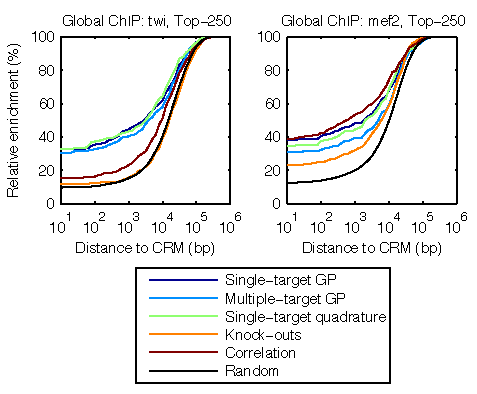
\includegraphics[width=3.5cm]{fig4.pdf}
\end{figure}
\centering

\end{columns}
}

%%%%%%%%%%%%%%%%%%%%%%%%%%%%%%%%%%%%%%%%%%%%%%%

%%%%%%%%%%%%%%%%%%%%%%%%%%%%%%%%%%%%%%%%%%%%%%%

\frame {
  \frametitle{Ranking assessment}

\centering
Changing the distance threshold  between CRM and positive targets


\centering
\begin{figure}
            \centering
            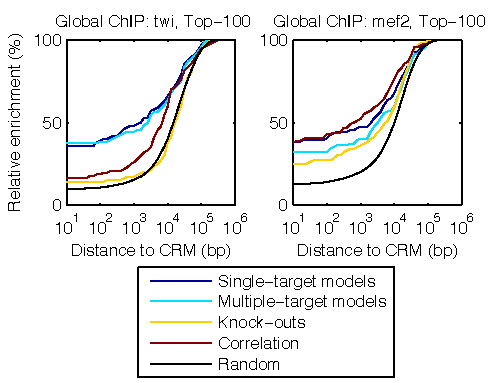
\includegraphics[width=6cm]{fig5.pdf}
	    
\end{figure}

}

%%%%%%%%%%%%%%%%%%%%%%%%%%%%%%%%%%%%%%%%%%%%%%%

\frame {
  \frametitle{Ranking assessment}

\centering
Changing the size of the dataset


\centering
\begin{figure}
            \centering
            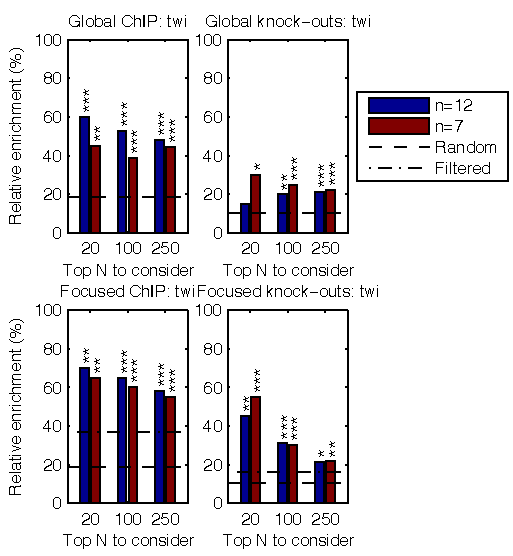
\includegraphics[width=5cm]{fig6.pdf}
	    
\end{figure}

}

%%%%%%%%%%%%%%%%%%%%%%%%%%%%%%%%%%%%%%%%%%%%%%%


%%%%%%%%%%%%%%%%%%%%%%%%%%%%%%%%%%%%%%%%%%%%%%%

\section{Current work and conclusion}
\subsection{Modelling combinatorial regulation}
\frame {
  \frametitle{Modelling combinatorial regulation}

Many target genes are regulated by multiple transcription factors

\centering
\begin{figure}
            \centering
            \includegraphics[width=9cm]{masamb10abs}
	    
\end{figure}

\pause
Network inference becomes much more challenging because the models become more complex and the space of models is huge.
}

\subsection{Conclusion}
\frame{ \frametitle{Conclusion}

\begin{itemize}
\item Gene regulatory networks are fundamental to understanding many cellular processes
\pause
\item Inference of gene regulatory networks requires input from multiple data sources \pause - these may be noisy and incomplete
\pause
\item Model-based inference can make effective use of these data, even when models are highly simplified
\pause
\item Gaussian processes provide a useful way to close an open system without introducing too many additional parameters
\pause
\item When models don't fit the data then we learn something \pause -- and then we need new models and new experiments
\end{itemize}
}

\subsection{Acknowledgements}
\frame{ \frametitle{Acknowledgements}
\begin{itemize}
\item Co-PIs: Neil Lawrence, Antti Honkela (HUT Finland)
\item Experimental data: Eileen Furlong group (EMBL Heidelberg)
\end{itemize}

\vspace{1cm}

Funded by EPSRC award ``Gaussian
  processes for systems identification with applications in Systems
  Biology'', PASCAL2 Network of Excellence and the Academy of Finland

}
%%%%%%%%%%%%%%%%%%%%%%%%%%%%%%%%%%%%%%%%%%%%%%%%%%%%%%%%%%%%%%%%%%%%%%%%%%%%%%%%%%%%%%%%%

\frame{ \frametitle{Advertisement}
\centering
\begin{figure}
            \centering
            \includegraphics[width=4.5cm]{cover.pdf}
	    
\end{figure}
}



\end{document}


